\textbf{Цель работы:} исследования свободных колебаний в колебательном контуре.

\textbf{В работе используются:} генератор импульсов, электронное реле, магазин сопротивлений, магазин ёмкостей, индуктивность, электронный осциллограф, унивенрсальный мост.

\section{Теоретическое введение}

\subsection{Последовательный $RLC$ контур}

Рассмотрим электрический контур, состоящий из последовательно соединённых конденстора $C$, катушки индуктивности $L$ и резистора $R$. Обозначим разность потенциалов на конденсаторе $U_C$, а ток, текущий в контуре, через $I$. Тогда

\begin{equation}
    L \dfrac{d^2I}{dt^2} + R\dfrac{dI}{dt} + \dfrac{I}{C} = 0
\end{equation}

Вводя обозначения $\gamma = \dfrac{R}{2L}$, $\omega_0^2=\dfrac{1}{LC}$, получим уравнение

\begin{equation}
    \ddot{I} + 2\gamma\dot{I} + \omega_0^2I = 0
\end{equation}

Общее решение этого уравнения имеет следующий вид:

\begin{equation}
    I = -\dfrac{U_0}{L\kappa}e^{-\gamma t}\text{sh}(\kappa t), 
\end{equation}

где $\kappa = \sqrt{\gamma^2 - \omega_0^2}$, $U_0 = U_C$ -- начальное напряжение на конденсаторе.

\subsection{Свободные затухающие колебания}

В случае, когда $\gamma < \omega_0$, имеем $\kappa = i\omega$, где $\omega = \sqrt{\omega_0^2 - \gamma^2}$ -- \textit{частоты свободных (собственных) колебаний}. Тогда ток

\begin{equation}
    I = -\dfrac{U_0}{L\omega}e^{-\gamma t}\sin(\omega t)
\end{equation}

затухает и имеет колебательный характер. Величина $\gamma$ определяет затухание колебаний: $\gamma = \dfrac{1}{\tau}$, где $\tau$ -- время затухание амплитуды в $e$ раз.
Формулы для наряжение на кондесаторе и тока в цепи можно переписать иначе:

\begin{equation}
    \begin{array}{c}
        U_C = U_0 \dfrac{\omega_0}{\omega}e^{-\gamma t} \cos(\omega t - \theta),\\
        \\
        I = -\dfrac{U_0}{L}e^{-\gamma t} \cos(\omega t - \theta).
    \end{array}
\end{equation}

\subsection{Апериодические колебания}

В случае $\gamma > \omega_0$, формулы для тока и напряжения на конденсаторе имеют следующий вид:

\begin{equation}
    \begin{array}{c}
        I = -\dfrac{U_0}{L\kappa}e^{-\gamma t}\text{sh}(\kappa t),\\
        \\
        U_C = U_0 e^{-\gamma t}\left( \dfrac{\gamma}{\kappa}\text{sh}(\kappa t) + \text{ch}(\kappa t) \right).
    \end{array}
\end{equation}

Процесс в этом случае не является колебательным, его называют апериодическим. Режим, соответствующий $\gamma = \omega_0$, называются \textit{критическим}. В этом случае предельный переход $\omega \rightarrow 0$ в $(6)$ даст 

\begin{equation}
    \begin{array}{c}
        I = -\dfrac{U_0}{L}te^{-\gamma t},\\
        \\
        U_C=U_0 e^{-\gamma t}(1+\gamma t).
    \end{array}
\end{equation}

Сопротивление в этом случае 

\begin{equation}
    R_{\text{кр}}= 2 \sqrt{\dfrac{L}{C}}
\end{equation}

называется \textit{критическим сопротивлением} контура.

\textit{Добротность} контура по определению 

\begin{equation}
    Q = 2\pi \dfrac{W}{\Delta W},
\end{equation}

где $W$ -- запасённая энергия, $\Delta W$ -- потери за период. Тогда

\begin{equation}
    Q = 2\pi\dfrac{CU_0^2/2 \cdot e^{-2\gamma t}}{CU_0^2/2 \cdot (e^{-2\gamma t} - e^{-2\gamma (T+t)})}=\dfrac{\pi}{\gamma T}=\dfrac{1}{R}\sqrt{\dfrac{L}{C}}.
\end{equation}

\textit{Логарифмическим декрементом затухания} называются число

\begin{equation}
    \Theta = \text{ln}\dfrac{U_k}{U_{k+1}}=\text{ln} e^{\gamma T}=\gamma T.
\end{equation}

или 

\begin{equation}
    \Theta = \dfrac{1}{n} \text{ln}\dfrac{U_k}{U_{k+n}}.
\end{equation}

\section{Экспериментальная установка}

\begin{figure}[h]
    \centering
    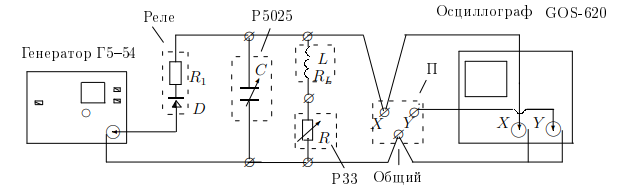
\includegraphics[width = 12 cm]{images/1.png}
    \caption{Экспериментальная установка}
    \label{eksp_ust}
\end{figure}


На рисунке приведена схема для исследования свободных колебаний в контуре, содержащем постоянную индуктивность $L$ и переменные ёмкость $C$ и сопротивление $R$. Колебания наблюдаются на экране осциллографа.

Для периодического возбуждения колебаний в контуре используется генератор импульсов Г5-54. С выхода генератора по коаксиальному кабелю импульсы поступают на колебательный контур через электронное реле, смонтированное в отдельном блоке (или на выходе генератора). Реле содержит тиристор $D$ и ограничительный резистор $R_1$.

Импульсы заряжают конденсатор $C$. После каждого импульса генератор отключается от колебательного контура, и в контуре возникают свободные затухающие колебания. Входное сопротивление осциллографа велико ($\approx 1$ МОм), так что его влиянием на контур можно пренебречь. 

Для получения устойчивой картины затухающих колебаний используется режим ждущей развёртки с синхронизацией внешними импульсами, поступающими с выхода <<синхроимпульсы>> генератора.

\section{Ход работы}

\subsection{Проверка формулы Томсона}

Установим в контуре $R = 0$, $C = 0,02$ мкФ. Для генератора импульсов имеем следующие настройки: длительность импульсов $5$ мкс, частота повторения импульсов $100$ Гц.

Увеличивая значение $C$, снимем зависимость $T(C)$:

\begin{table}[h!]
    \centering
    \begin{tabular}{|c|r|r|r|r|r|r|}
    \hline
    \textbf{$T$, мкс} & 350  & 425  & 540  & 740  & 940  & 1240 \\ \hline
    \textbf{$C$, мкФ} & 0,02 & 0,03 & 0,05 & 0,09 & 0,15 & 0,25 \\ \hline
    \textbf{$T$, мкс} & 1460 & 1660 & 1850 & 2000 & 2150 & 2300 \\ \hline
    \textbf{$C$, мкФ} & 0,36 & 0,47 & 0,58 & 0,69 & 0,80 & 0,90 \\ \hline
    \end{tabular}
\end{table}

Считая, что сопротивление цепи равно нулю, посчитаем также теоретические значение периодов по формуле Томсона. Для этого снимем значение индуктивности катушки: $L = 145 \pm 1$ мГн (при рассматриваемом диапазоне частот). С помощью посчитанных значений построим таблицу, а затем график $T_{\text{теор}}(T_{\text{эксп}})$:

\begin{table}[h!]
    \centering
    \begin{tabular}{|c|r|r|r|r|r|r|}
    \hline
    \textbf{$T$, мкс} & 344,14 & 421,48 & 544,13 & 730,04 & 942,47 & 1216,73 \\ \hline
    \textbf{$C$, мкФ} & 0,02   & 0,03   & 0,05   & 0,09   & 0,15   & 0,25    \\ \hline
    \textbf{$T$, мкс} & 1460   & 1660   & 1850   & 2000   & 2150   & 2300    \\ \hline
    \textbf{$C$, мкФ} & 0,36   & 0,47   & 0,58   & 0,69   & 0,8    & 0,9     \\ \hline
    \end{tabular}
\end{table}

\begin{figure}[h!]
    \centering
    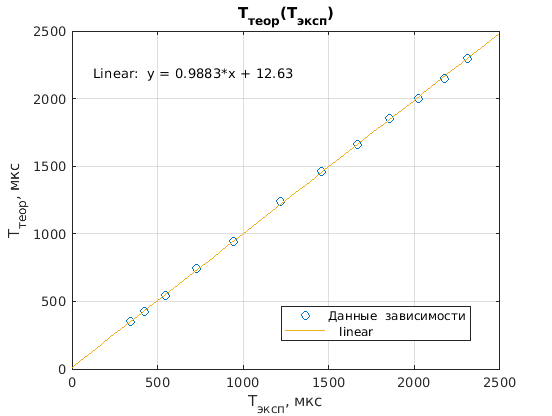
\includegraphics[width = 12 cm]{images/exp1.png}
    \caption{График зависимости $T_{\text{теор}}(T_{\text{эксп}})$}
    \label{exp1}
\end{figure}

Из графика видно, что для цепи с $R = 0$ действительно выполняется формула Томсона для периода свободных колебаний. Однако нужно учитывать, что у катушки всё ещё есть сопротивление $R_L$ и формула Томсона описывает период колебаний лишь приблизительно.

\subsection{Определение критического сопротивления}

Из формулы Томсона, имея значение индуктивности катушки, найдём такую ёмкость, при которой частота колебаний будет равна $5$ кГц: $C = 6,75 \pm 0,08$ мкФ. Тогда поставим значение $C = 6,7$ мкФ на магазине. Из полученных значений найдём критическое сопротивление из теоретической формлулы: $R_{\text{кр}} = 2 \sqrt{L/C} = 9430 \pm 30$ Ом.

Теперь найдём значение критического сопротивления, увеличивая сопротивление на магазине от нуля до тех пор, пока колебания не станут апериодическими: $R_{\text{кр}} = 9000 \pm 100$ Ом.

Теперь установим посчитанное значение ёмкости на магазине ёмкостей. Снимания значения амплитуд с осциллографа, посчитаем зависимость логарифмического декремента затухания от сопротивления $\theta (R)$, учитывая, что при рассматриваемой частоте колебаний у катушки сопротивление $R_L = 17,2 \pm 0,05$ Ом (это значение нужно добавить к сопротивлению магазина сопротивлений):

\begin{table}[h!]
    \centering
    \begin{tabular}{|c|l|l|l|l|l|l|l|l|}
    \hline
    \textbf{$\theta$} & 0,57 & 0,69 & 0,88 & 0,96 & 1,10 & 1,41 & 1,67 & 1,76 \\ \hline
    \textbf{$R$, Ом}  & 917  & 1117 & 1367 & 1617 & 1817 & 2267 & 2517 & 2717 \\ \hline
    \end{tabular}
\end{table}

Построим график $\theta (R)$:

\begin{figure}[h!]
    \centering
    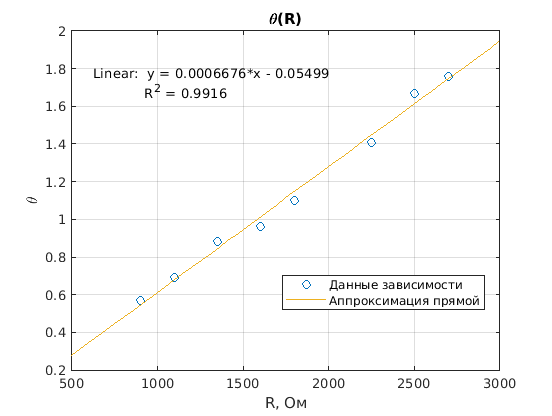
\includegraphics[width = 12 cm]{images/exp2.png}
    \caption{График зависимости $\theta (R)$}
    \label{exp2}
\end{figure}

Зависимость действительно линейная, как и описывает теория. Теперь построим зависимость $\frac{1}{\theta^2}(\frac{1}{R^2})$:

\begin{figure}[h!]
    \centering
    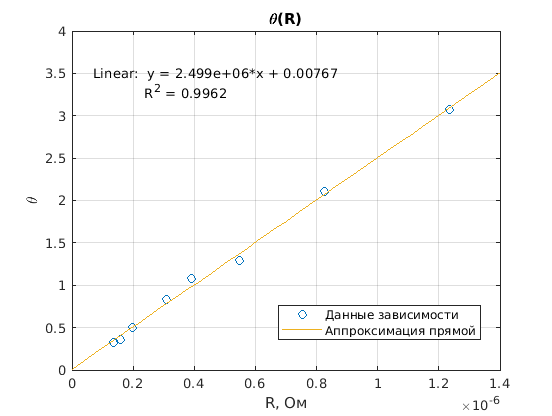
\includegraphics[width = 12 cm]{images/exp3.png}
    \caption{График зависимости $\frac{1}{\theta^2}(\frac{1}{R^2})$}
    \label{exp3}
\end{figure}


Коэффициент наклона равен $k = (2,50 \pm 0,13) \cdot 10^6 \; \text{Ом}^{-2}$, при этом критическое сопротивление связано с этим коэффициентом формулой $R_{\text{кр}} = 2 \pi \sqrt{k} = 9930 \pm 260$ Ом.

Таким образом, измеренное значение критического сопротивления тремя способами оказалось во всех случаях примерно одинаковым.

\subsection{Добротность контура}

Рассчитаем теперь значения добротности для минимум и максимума логарифмического декремента, взятые из предыдущей таблицы с данными:

\begin{equation}
    Q_{min} = \frac{\pi}{\theta_{max}} = 1,79 \pm 0,10, \;
    Q_{max} = \frac{\pi}{\theta_{min}} = 5,51 \pm 0,33
\end{equation}

Погрешности высоки из-за погрешностей измерения лоарифмических декрементов затухания.

Теперь найдём те же самые значения через спирали на фазовой плоскости, измеряя аналогично логарифмический декремент затухания:

\begin{equation}
    Q_{min} = \frac{\pi}{\theta_{max}} = 1,82 \pm 0,08, \;
    Q_{max} = \frac{\pi}{\theta_{min}} = 5,57 \pm 0,29
\end{equation}

\section{Заключение}

В результате эксперимента подтверждена формула Томсона для свободных колебаний, а так же измерены различные параметры $RLC$ контура при различных значениях параметров контура.

Ёмкость катушки фиксирована на протяжении всего эксперимента и при частоте в районе $5000$ Гц равна $L = 145,1 \pm 0,2$ мГн, для конденсатора имеем $C = 6,7$ мкФ.

Критическое сопротивление для контура было найдено тремя способами: $R_{\text{кр}} = 9430 \pm 30$ Ом -- посчитанное значение из теоретической формулы, $R_{\text{кр}} = 9000 \pm 100$ Ом -- напрямую, исследуя, когда колебания переходят в апериодические и $R_{\text{кр}} = 9930 \pm 260$ Ом -- значение, найденное косвенным способом через измерение логарифмических декрементов затухания при различных сопротивлениях. Таким образом, самое точное значение -- измеренное через формулу. При этом все значения получились одинаковыми в пределах нескольких $\sigma$.

Для добротностей имеем следующее: $Q_{min} = 1,79 \pm 0,10$, $Q_{max} = 5,51 \pm 0,33$ -- значения, измеренные через логарифмические декременты затухания из ранее построенной таблицы,  $Q_{min} = 1,82 \pm 0,08$, $Q_{max} = 5,57 \pm 0,29$ -- значения, измеренные через спирали на фазовой диаграмме. Таким образом, значения совпадают, но в методе фазовой диаграммы значения имеют меньшую погрешность.
